\documentclass[review]{elsarticle}

\usepackage{lineno,hyperref}
\usepackage[doublespacing]{setspace}
\usepackage{float}
\usepackage{graphicx,enumitem}
\usepackage{xcolor}
\modulolinenumbers[5]
\newcommand{\tss}{\textsuperscript}
\newcommand{\tsbs}{\textsubscript}
\graphicspath{{images/}}
\journal{Journal of Applied Radiation and Isotopes}


%%%%%%%%%%%%%%%%%%%%%%%
%% Elsevier bibliography styles
%%%%%%%%%%%%%%%%%%%%%%%
%% To change the style, put a % in front of the second line of the current style and
%% remove the % from the second line of the style you would like to use.
%%%%%%%%%%%%%%%%%%%%%%%

%% Numbered
%\bibliographystyle{model1-num-names}

%% Numbered without titles
%\bibliographystyle{model1a-num-names}

%% Harvard
%\bibliographystyle{model2-names.bst}\biboptions{authoryear}

%% Vancouver numbered
%\usepackage{numcompress}\bibliographystyle{model3-num-names}

%% Vancouver name/year
%\usepackage{numcompress}\bibliographystyle{model4-names}\biboptions{authoryear}

%% APA style
%\bibliographystyle{model5-names}\biboptions{authoryear}

%% AMA style
%\usepackage{numcompress}\bibliographystyle{model6-num-names}

%% `Elsevier LaTeX' style
\bibliographystyle{elsarticle-num}
%%%%%%%%%%%%%%%%%%%%%%%

\begin{document}

\begin{frontmatter}

\title{Fission Product Decontamination Factors for Plutonium Separated by PUREX from above
	   Low Burn-up, fast-neutron irradiated Depleted UO\tsbs{2}}

%% Group authors per affiliation:
\author[NSSPI,NUEN]{Paul M. Mendoza}

\author[NSSPI,NUEN]{Sunil S. Chirayath\corref{mycorrespondingauthor}}
\cortext[mycorrespondingauthor]{Corresponding author}
\ead{sunilsc@tamu.edu}

\author[CYC]{Charles M. Folden III}

\address{Texas A\&M University, College Station, TX 77843-3473}

\address[NSSPI]{Nuclear Security Science \& Policy Institute (NSSPI)}
\address[NUEN]{TAMU Department of Nuclear Engineering}
\address[CYC]{Cyclotron Institute}

\begin{abstract}
\begin{singlespace}
Experimental investigations to determine fission product (FP) separation from actinides
(U and Pu) while employing the Plutonium Uranium Redox Extraction (PUREX)
 process to purify plutonium produced in a fast neutron irradiated depleted uranium dioxide (DUO\tsbs{2})
 target were conducted.
 The sample was a DUO\tsbs{2} surrogate pellet (0.2562 wt.\% \emph{initial} \tss{235}U)
 irradiated to a low-burn-up (4.43 $\pm$ 0.31 GWd/tHM) that was PUREX process 538
 days after neutron irradiation. 
 Decontamination factors (DF) for elements
 U, Mo, Ru, Ce, Sm, Sr, Pm, Eu, Nd, Pd, Cd, Ba and Sn
 for two PUREX experiments using 30 vol.\% tri-n-butyl phosphate in a kerosene diluent
 with less than 0.3\% uranium saturation in 4 M nitric acid were determined. The first experiment
 characterized Pu DFs for a single contact extraction and back-extraction while the 
 second had multiple contacts for larger product recovery. The bench-top scale
 PUREX process had an overall 76\% and 94\% Pu recovery and an overall activity decontamination
 factor of \color{red}20 \color{black} and \color{red}5 \color{black} for the first 
 and second experiments respectfully.
\end{singlespace}
\end{abstract}

\begin{keyword}
\texttt{PUREX\sep Decontamination Factor\sep Depleted Uranium} 
\MSC[2010] 00-01\sep  99-00
\end{keyword}

\end{frontmatter}

\linenumbers

\section{Introduction}

\paragraph{Background} In a recent publication, our group suggested that investigation
 of PUREX-processed plutonium for trace contaminates could give indication of material 
 origins, but that a broad study of many elements would be necessary \cite{chirayath2015}.
 Descriptions of various PUREX processes are provided in many sources \cite{reas1957,stoller1961,benedict1982}
 with explanations of chemistry including flow sheets and DF values, while additional sources provide 
 other DFs  for PUREX \cite{gresky1950,arker1954,chandler1954}.
 These sources generally report overall beta or gamma DFs of up to ~10\tss{8} with Pu recoveries
 of 99.7\% for industrial-scale reprocessing facilities.

 While distribution coefficients (DC) for 
 the various process separation steps of PUREX have been previously reported, details about 
 elemental DFs for PUREX cycles have been largely limited to the major activity contributors,
 such as \tss{106}Ru and \tss{95}Zr \cite{stoller1961}. 
 A compilation of distribution data for PUREX extraction processes provide DC
 information for U, Th, and Pu in a variety of concentrations \cite{prout1957}.
 DCs for Zr, rare earth metals, Pu, and Th are also available \cite{alcockbed1957,
 best1957,hesford1957,scargil1957,alcock1958,best1959,hesford1959}
 
 Although a DC (coupled with process information) can be used to calculate a reasonable estimate of DF 
 \cite{colburn1939,sherwood1952,long1967,perry2008},variability of DCs under different
 system conditions give rise to uncertainty in calculated results.
 For example, DCs between tri-n-butyl phosphate (TBP) and nitric acid (HNO3) have 
 been reported for U, Pu, Zr, Nb, Ru, and the rare earth elements, but vary with 
 nitric acid concentration and uranium saturation in TBP \cite{sherwood1952,stoller1961}.
 These sources also derive mathematical correlations between DC and DF, but experimental 
 PUREX DFs for a large number of individual elements were not provided. 
 Additionally, gallium has been 
 studied for separation \cite{collins2000} because it is a common contaminate in weapons
 grade Pu. 
 
 In the current work, a 12.9 mg of DUO\tsbs{2} 
 was irradiated in a pseudo-fast neutron spectrum at the High Flux isotope Reactor 
 at Oak Ridge National Laboratory. The DUO\tsbs{2} pellet, containing FP and weapons-grade
 Pu, was dissolved into a nitric acid solution and subjected to two different PUREX experiments
 for DF characterization and Pu product recovery.
 Solutions were analyzed at each step with Inductively Coupled Plasma-Mass Spectrometry (ICP-MS).
 The experimental work used bench-top-scale methods to isolate a large fraction of Pu,
 measure DFs for fission products, and measure gamma DFs as part of a larger project to 
 develop forensic radio-analytical capabilities at Texas A\&M University.
 
\paragraph{Terminology} A DCs is defined as the concentration ratio between the
 organic (“org”) and aqueous (“aq”) phases as shown in Equation \ref{eq:1},
 and describes the steady-state distribution of any species in the system during 
 PUREX separation processes \cite{benedict1982}:

 \begin{equation}\label{eq:1}
DC=\frac{c_{org}}{c_{aq}}
 \end{equation}
 
 where $c$ is the concentration of the specific species in the indicated phase. 
 DCs are specific to an element and vary widely with the concentration and
 temperature of the solvents. They are also affected by saturation of uranium
 and plutonium in the system and time since preparation of the solution 
 \cite{stoller1961,michael2010}. For PUREX, the fraction of mass
 $f_{org}$ deposited in the organic (TBP) phase for a single element 
 (assuming equal contact volumes) is given by Equation \ref{eq:2}.
 
\begin{equation}\label{eq:2}
f_{org}=(1+DC^{-1})^{-1}
\end{equation}
  
 After several cycles of plutonium extraction/decontamination are complete, 
 the measured effectiveness of a PUREX cycle is described by the DF, which is 
 fundamentally determined by DCs and measure the effectiveness with which a 
 contaminant, $j$, is removed from a product. In this work, the product of interest
 is plutonium, and the DF is defined by Equation \ref{eq:3}.
 
 \begin{equation}\label{eq:3}
DF_j=\frac{\left\frac{c_j}{c_{Pu}}\right|_{initial}}{\left\frac{c_j}{c_{Pu}}\right|_{final}}
\end{equation}
 
 $Initial$ and $final$ refer to the values before and after purification, respectively. 
 DFs are also characteristic of different process cycles, and may have larger values
 ($>$ 10\tss{7}) for industrial scale PUREX compared to the bench-top scale version presented here
 \cite{stoller1961,benedict1982}.  
 
 Industrial processes report either an overall DF value, or a DF value for a single isotope. 
 What is needed for forensics purposes is DFs for individual FP contaminants, which is why elemental
 DF values were obtained for bench-top-scale PUREX process performed on a DUO\tsbs{2} 
 surrogate sample. 
 
\section{Experiment}

A commercially acquired pellet containing 12.9 $\pm$ 0.1 mg of DUO\tsbs{2} was irradiated over the 
course of three months with two shut down periods in the HFIR flux spectrum to 4.43 $\pm$ 0.31
GWd/tHM \cite{swinney}. The burn-up was determined by measuring the \tss{137}Cs activity. This produced 
0.237 $\pm$ 0.008 mg of Pu. After the short lived radioisotopes had opportunity to decay, 
the irradiated pellet was shipped to Texas A\&M University, counted with a standard
Canberra electrode coaxial Ge detector to determine relative activity, and transferred to a round-bottom
 flask.

Samples were prepared as shown in Figure \ref{fig:diss}, and described below. 5.0 ml of 8 M HNO\tsbs{3} was added to the flask, which was heated to 50 $^{\circ}$C
 with constant 100 rpm stiring for two hours. This solution will be referred to as the 
 ``dissolution solution''.
			\begin{figure}[h!]
				\centerline{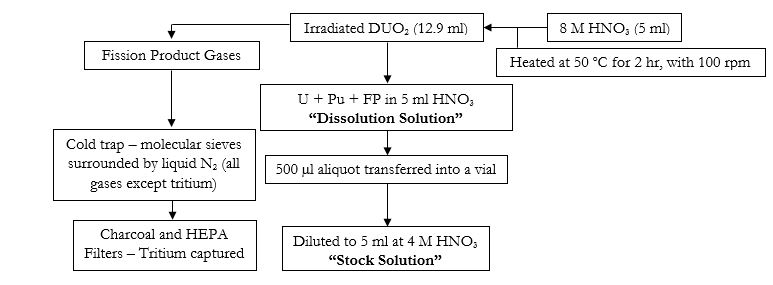
\includegraphics[scale=0.65]{dissolution}}
				\caption{Flow chart for dissolution.}
				\label{fig:diss}
			\end{figure}
 The flask was connected to a cold trap with the help of a Schlenk 
 line. The fission product gases such as H\tsbs{2}, CO\tsbs{2}, Kr, Br, I and N\tsbs{2}O
 were captured in a cold trap containing molecular sieves that were chilled by liquid nitrogen.
 In order to reduce the amount of activity per sample, 500 $\mu l$ from the dissolution solution
 was diluted to 5.0 ml and the concentration was changed to 4 M HNO\tsbs{3}. From this solution, 
 referred to as the ``stock solution'', 0.5 ml aliquotes, containing $\sim$1\% of the pellet, were
 used in bench-top-scale PUREX experiments described in the two subsections below.
 The activity concentration of the stock solution was approximately 80 \mu Ci/ml.
 
Experiments started with transferring a 500 $\mu l$ aliquot of stock solution 
and 0.5 mg of NaNO\tsbs{2} to a 15 ml centrifuge tube. The tube was subsequently stirred and covered to retain the resulting NO\tsbs{2} gas.
The solution was left overnight so that NO\tsbs{2} gas completely oxidized Pu(III) to Pu(IV).
During extraction and back-extraction, both experiments had the aqueous and organic phases
mixed on a vortex mixer for 15 minutes at 1500 rpm, after which the two phases were allowed to settle and separate.
The phases were physically separated into two different vials through careful pipetting. 

Each extraction and back-extraction mixed organic and aqueous mixtures with unequal volumes. 
The solution being added always contained an extra 200 $\mu l$ to reduce the chance of accidentally
pipetting HNO\tsbs{3}. For example, if TBP were being added to the stock solution described above,
700 $\mu l$ would be added initially and 500 $\mu l$ removed. This excess volume will be later referenced
as hold-up volume. 
 
The kerosene (100\%) and sodium nitrite (100\%) used for these experiments were acquired from
sciencelab.com \cite{sciencelab}, 69\% nitric acid was acquired from Mallinckrodt Chemicals \cite{mal}, Tri-n-butyl phosphate
($>$99\%) was acquired from Fisher Scientific \cite{fish}, and iron sulfamate (40.26\%) was acquired from Strem Chemicals
Incorporation \cite{strem}. 

The pellet, both prior to dissolution and after, was counted with a Canberra HPGe detector model
number CC4018 which was connected to a Canberra Lynx MCA \cite{hpge,lynx}. Canberra's software package GENIE-2000 version
3.2.1 \cite{version19952} was used to collect spectra with samples inside a lead tomb.
The same detector was used to count the various process solutions. 
Inductively coupled plasma mass spectrometry (ICP-MS) was also conducted for aqueous 
samples using a PerkinElmer NexION 300X quadrupole ICP-MS \cite{MS}.


\paragraph{First Experiment} The purpose of the first experiment was to quantify product
 recovery and DF values for a single contact extraction and back-extraction of Pu. 
U(VI) and Pu(IV) were extracted and decontaminated by contacting the prepared stock solution 
with a solution of 30 vol.\% TBP with a kerosene diluent. After mixing, and separation of the 
two phases, Pu(IV) was reduced to Pu(III) and back-extracted by contacting the removed TBP
solution with 0.75 M HNO\tsbs{3} in a 0.024 M ferrous sulfamate solution via oxidation of Fe(II).  
The stock solution both before and after TBP contact, as well as the final solution containing 
back-extracted Pu, were analyzed with ICP-MS. 
\paragraph{Second Experiment} The purpose of the second experiment was to extract a large fraction
 of Pu. Utilizing the results from the first experiment, it was determined that
 contacting the prepared stock solution four times with TBP would extract over 90\% of the Pu. 
 Therefore, this experiment had four TBP contacts with the prepared stock solution. The TBP was
 then collected into a single vial, and contacted three times with the ferrous sulfamate solution.

 In order to ensure minimal U back-extraction, the HNO\tsbs{3} concentration for this experiment was increased to 4 M because $NO_3^-$ concentrations
affect the distribution ratio for U. Higher HNO\tsbs{3} concentrations reduce the degree to which
U is back-extracted \cite{stoller1961}. Three contacts of the ferrous sulfamate solution ensured
complete back-extraction of Pu, while the higher nitric acid concentration minimized back-extraction of U.
 The same solutions as described in the first experiment
were analyzed with ICP-MS.
The final back-extracted Pu solution underwent the 4 extraction 3 back-extraction process once more to
verify the repeatability of the process and for comparison
with the first extraction/back-extraction cycle. The final solution Pu was reset with the 
addition of 0.5 mg of NaNO\tsbs{2} to convert all the Pu(III) to Pu(IV).  


\section{Results}

The Pu recovery for the first and second experiments are shown in Table \ref{tab:UPu}.
For experiment 1, the amount of U recovery was much higher than for experiment 2, even with multiple 
contacts. This is due to the different HNO\tsbs{3} concentrations for the back-extraction solutions
between the two experiments, as described earlier.
The second experiment second cycle had a 90\% Pu recovery with 
an 95\% of the remaining U left in the organic phase. The reason the second cycle did not perform as well
as the first was due to Fe(II) catalytically oxidizing to Fe(III) with $NO_2^-$ \cite{stoller1961}.

The DCs for U and Pu were 37.2 $\pm$ 5.3 and 16.2 $\pm$ 2.3, respectfully,
which indicate that large fractions of the U and Pu were removed from stock solutions. 
Using Equation \ref{eq:2}, which assumes equal volumes,
 with these two DC values, over 99.99\% of the U and Pu should be
extracted, with nearly all of the Pu being back-extracted. The reason for lower recovery values
is due to hold-up volumes left in the extraction/back-extraction vials \cite{long1967}.
This is be further explained in the next section. 

\begin{table}[ht]
\caption{Recoveries of U and Pu for the different experiments}
\label{tab:UPu}
\centering
\begin{tabular}{rlrrrr}
  \hline
 \multicolumn{1}{|c|}{}& \multicolumn{1}{|c}{Pu Recovery} & $\pm$ & \multicolumn{1}{|c}{U Recovery} & \multicolumn{1}{c|}{$\pm$} \\ 
  \hline
   \multicolumn{1}{|c|}{Experiment 1}         & 76\%    & \multicolumn{1}{c|}{0.30\%} & 25\%    & \multicolumn{1}{c|}{0.03\%} \\ 
   \multicolumn{1}{|c|}{Experiment 2 Cycle 1} & 94\%    & \multicolumn{1}{c|}{0.90\%} & 7\%     & \multicolumn{1}{c|}{0.06\%} \\ 
   \multicolumn{1}{|c|}{Experiment 2 Cycle 2} & 90\%    & \multicolumn{1}{c|}{0.60\%} & 5\%     & \multicolumn{1}{c|}{0.10\%} \\ 
   \multicolumn{1}{|c|}{Experiment 2 Cycles 1\&2} & 85\% & \multicolumn{1}{c|}{0.99\%} &0.35\% & \multicolumn{1}{c|}{0.08\%} \\
   \hline
\end{tabular}
\end{table}


The DF calculations utilized concentration ratios between contaminants that were normalized
to the Pu so that volume changes due to processing were negated, as shown in Equation \ref{eq:3}. 
Both the first and second experiment first cycle DF values
are shown in Table \ref{tab:DF}. It should be noted that the Ba calculation 
utilized \tss{138}Ba with
background Ba subtracted; the background was 
determined with \tss{134}Ba, and is subject to very
high errors due to the low amounts of \tss{134}Ba in the system.


\begin{table}[ht]
\caption{Decontamination factors for single and multiple contact PUREX}
\label{tab:DF}
\centering
\begin{tabular}{rlrrrrrl}
  \hline
 \multicolumn{1}{|c|}{Element} & Exp 1 & $\pm$ & \multicolumn{1}{|c}{Exp 2} & $\pm$ & \multicolumn{1}{|c|}{Isotopes Used} \\ 
  \hline
  \multicolumn{1}{|c|}{Rb}  & 32     & 1.55   & \multicolumn{1}{|c}{1.84 } & 0.26  & \multicolumn{1}{|c|}{\tss{85}Rb} \\ 
  \multicolumn{1}{|c|}{Sr}  & 233.5  & 12.74  & \multicolumn{1}{|c}{38.26} & 2.23  & \multicolumn{1}{|c|}{\tss{90}Sr}\\ 
  \multicolumn{1}{|c|}{Mo}  & 20.67  & 2.03   & \multicolumn{1}{|c}{1.19 } & 0.25  & \multicolumn{1}{|c|}{\tss{97}Mo}\\ 
  \multicolumn{1}{|c|}{Ru}  & 49     & 1.90   & \multicolumn{1}{|c}{2.84 } & 0.11  & \multicolumn{1}{|c|}{\tss{101,102,104}Ru} \\ 
  \multicolumn{1}{|c|}{Pd}  & 65     & 14.3   & \multicolumn{1}{|c}{3.62 } & 0.94  & \multicolumn{1}{|c|}{\tss{108,110}Pd} \\ 
  \multicolumn{1}{|c|}{Cd}  & 61     & 6.60   & \multicolumn{1}{|c}{3.50 } & 0.98  & \multicolumn{1}{|c|}{\tss{112}Cd}\\ 
  \multicolumn{1}{|c|}{Sn}  & 7.45   & 0.43   & \multicolumn{1}{|c}{13.85} & 1.29  & \multicolumn{1}{|c|}{\tss{119}Sn}\\ 
  \multicolumn{1}{|c|}{Cs}  & 146    & 7.58   & \multicolumn{1}{|c}{11.92} & 0.96  & \multicolumn{1}{|c|}{\tss{133}Cs}\\ 
  \multicolumn{1}{|c|}{Ba}  & 344    & 200    & \multicolumn{1}{|c}{0.39 } & 50    & \multicolumn{1}{|c|}{\tss{134,138}Ba}\\ 
  \multicolumn{1}{|c|}{Ce}  & 35.24  & 1.68   & \multicolumn{1}{|c}{3.2  } & 0.67  & \multicolumn{1}{|c|}{\tss{140,142}Ce}\\ 
  \multicolumn{1}{|c|}{Nd}  & 16.37  & 0.65   & \multicolumn{1}{|c}{5.94 } & 2.01  & \multicolumn{1}{|c|}{\tss{143}Nd} \\ 
  \multicolumn{1}{|c|}{Pm}  & 10.70  & 0.66   & \multicolumn{1}{|c}{3.3  } & 0.50  & \multicolumn{1}{|c|}{\tss{147}Pm}\\ 
  \multicolumn{1}{|c|}{Sm}  & 9.94   & 0.25   & \multicolumn{1}{|c}{2.5  } & 0.19  & \multicolumn{1}{|c|}{\tss{151}Sm}\\ 
  \multicolumn{1}{|c|}{Eu}  & 8.40   & 0.49   & \multicolumn{1}{|c}{2.6  } & 0.23  & \multicolumn{1}{|c|}{\tss{154}Eu}\\ 
  \multicolumn{1}{|c|}{U }  & 6.85   & 0.46   & \multicolumn{1}{|c}{15.08} & 0.60  & \multicolumn{1}{|c|}{\tss{238}U}\\ 
   \hline
\end{tabular}
\end{table}

The common trend is that the DF gets worse from the first experiment to the second. The major exception is
U, which has a better DF value. This is expected due to the change in HNO\tsbs{3} concentration 
in the iron sulfamate solution, and has been explained previously. The rest of the elements have worse 
DF values because of multiple contacts, and are low in general
because of the volume difference between the phases and hold-up volumes. 

\paragraph{Volumes Differences and Multiple Contacts}
An excellent description for how hold-up volumes decrease DF values is given in
\cite{long1967}, in the differential extraction section. In short, if TBP is used to extract
Pu, and if some TBP is left in contact with the nitric acid as hold-up, then some Pu will be lost.

Another reason why the DF values were lower than industrially reported values is due to the 
fact that the volume ratio of aqueous and organic phase was less than unity. 
If Equation \ref{eq:2} were rewritten to include the volume ratio between the aqueous
and organic phase, $V_R$, then the fraction of mass that passes to the organic phase
, $f_{org}$, would be given by Equation \ref{eq:4}.

\begin{equation}\label{eq:4}
f_{org}=(1+DC^{-1}V_R)^{-1}
\end{equation}

If the aqueous 
phase volume is less than the organic phase volume, then a larger percentage of contaminant will
pass into the organic phase. More Pu(IV) and U(VI) will also be extracted, but since their DC values
are large, the effect is not as tangible as for the fission products, with DC values below one. 
This effect is shown in Figure \ref{fig:TBP}, where theoretical DFs for the extraction step is shown
as a function of volume ratio and number of contacts.

Figure \ref{fig:TBP} shows how DF decreases with increasing volume of TBP and with with the number
contacts. The number of contacts decreases DF because less and less product is removed with each
extraction, while the amount of contaminant removed is about the same. 

\begin{figure}[h!]
	\centerline{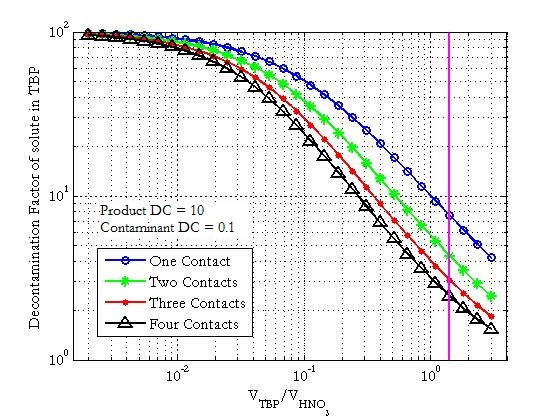
\includegraphics[scale=0.75]{TBP}}
	\caption{DFs as a function of volume ratios for the first to fourth contact in TBP.}
	\label{fig:TBP}
\end{figure}

Using equations described previously, the DF for both
experiments can be calculated with the assumption that the DC for both the extraction and back-extraction
are equal. Simulating these experiments and plotting DC versus DF is 
shown in Figure \ref{fig:four}.
The ratio of the DF for the second experiment and first is about 0.30.  
Which means that the second experiment DF value should be no better than 30\% of the first experiment. 
Looking back to Table \ref{tab:DF}, the ratio of the DF values between the second and first 
experiments, excluding U, is 0.27, with values above and below. 

\begin{figure}[h!]
	\centerline{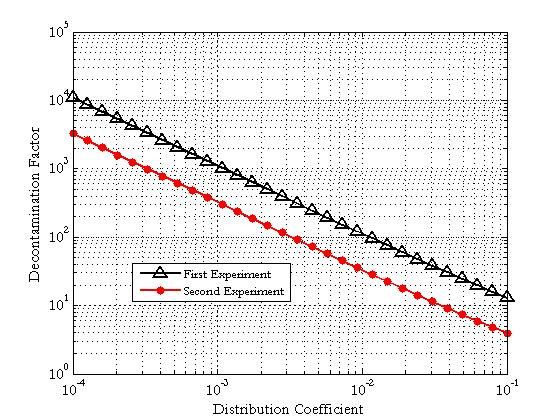
\includegraphics[scale=0.6]{four_contact}}
	\caption{Decontamination factors as a function of Distribution Coefficient for the first and second experiment.}
	\label{fig:four}
\end{figure}




\section{Conclusions}
Two experiments were conducted to quantify DF values for a variety of elements as well as 
extract a large fraction of Pu. It was determined that the volume ratio between organic 
and aqueous phases in extraction have an impact on DF values, and that multiple extraction
steps lead to large product recovery, but can also decrease DF values.
Future experiments will utilize a scrubbing stage in the PUREX process.




\cite{Feynman1963118,Dirac1953888}.

\section*{References}

\bibliography{mybibfile}

\end{document}